\section{Results}\label{sec:results}
% Include subsection showing the inventory for both cases maybe

\subsection{Manufacturing Impact}\label{subsec:results_manufacturing}
As mentioned in the previous section, first, the manufacturing processes for both note-taking approaches are compared. For this, the previously mentioned scenarios including their waste treatments are considered. 

As a first step, their effects per impact category were compared. Figure~\ref{fig:characterization_manufacturing} depicts a relative analysis for the most significant categories between both scenarios while Figure~\ref{fig:characterization_table_manufacturing} shows all absolute values for each category in either species per year, disability-adjusted life years (DALY) or in excess costs in 2013 US Dollars.


\begin{figure}[H]
    \centering
    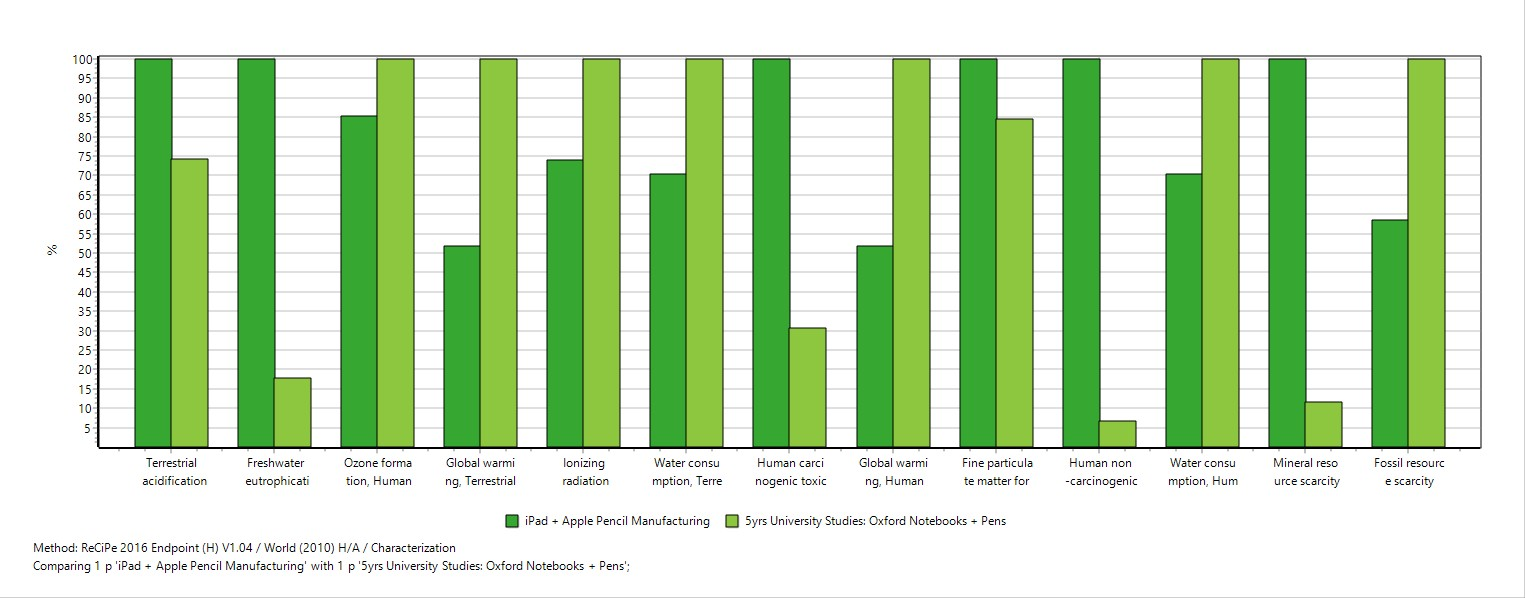
\includegraphics[width=\textwidth]{images/Manufacturing/Characterization_Manufacturing.JPG}
    \caption{Relative characterization for the manufacturing of the investigated note-taking approaches per impact category.}\label{fig:characterization_manufacturing}
\end{figure}

\begin{figure}[H]
    \centering
    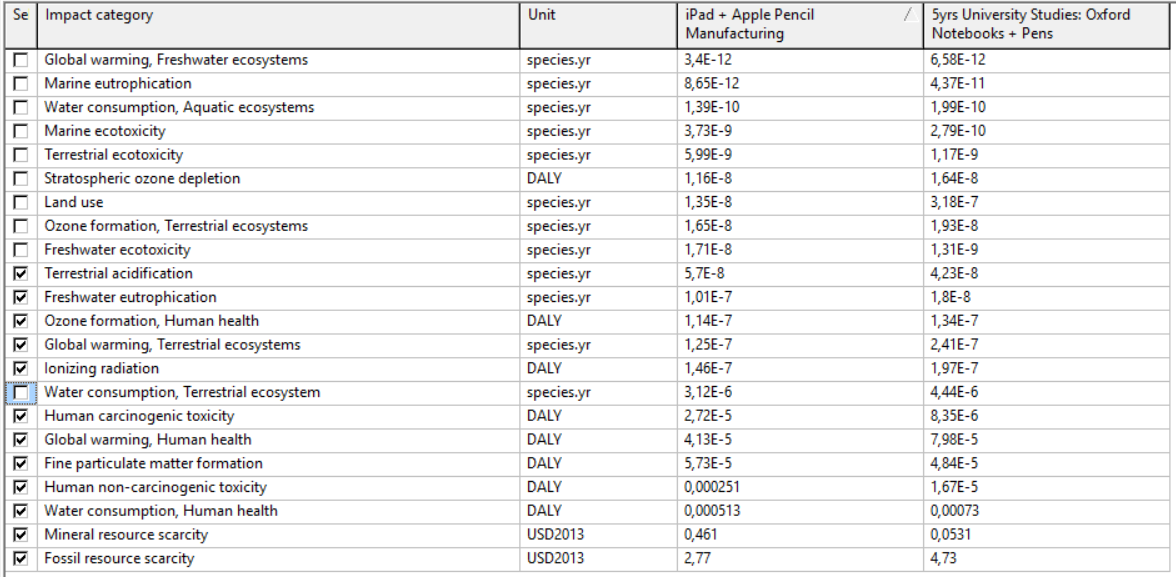
\includegraphics[width=0.9\textwidth]{images/Manufacturing/Characterization_Table_Manufacturing.PNG}
    \caption{Absolute characterization for the manufacturing of the investigated note-taking approaches per impact category.}\label{fig:characterization_table_manufacturing}
\end{figure}

\begin{figure}[H]
    \centering
    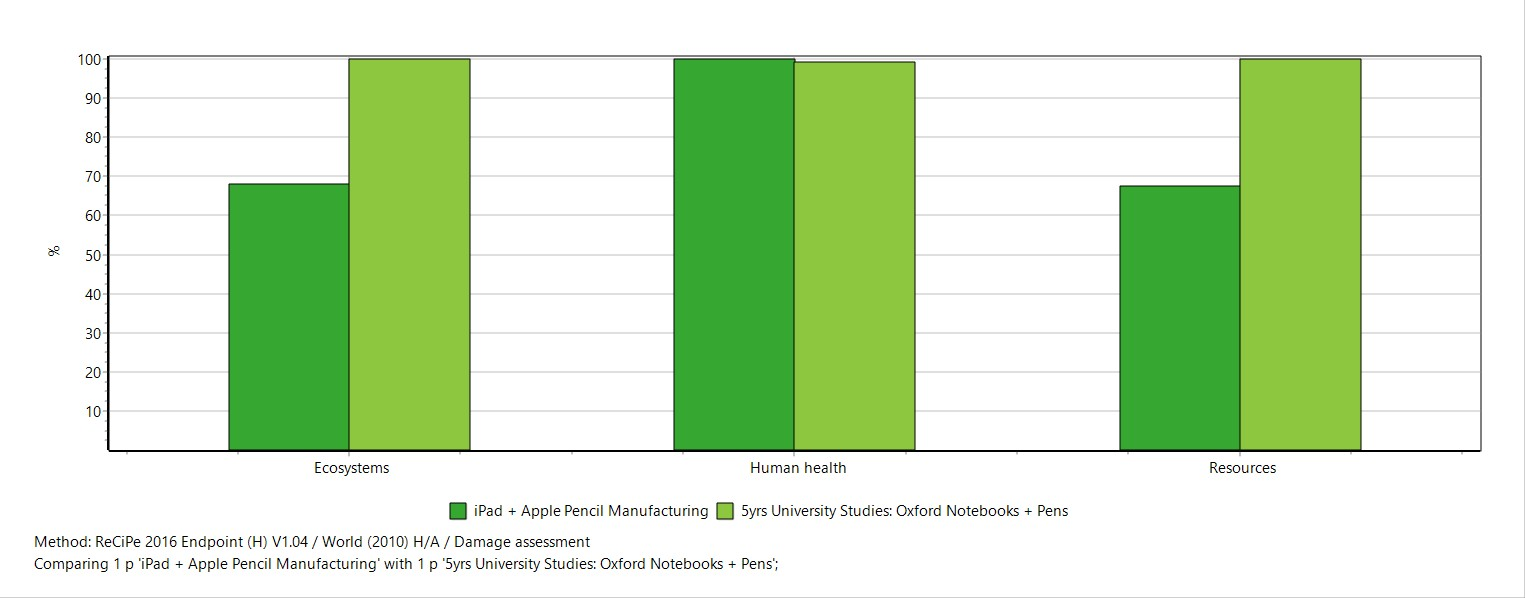
\includegraphics[width=\textwidth]{images/Manufacturing/Damage_Assessment_Manufacturing.JPG}
    \caption{caption}\label{fig:damage_assessment_manufacturing}
\end{figure}

\begin{figure}[H]
    \centering
    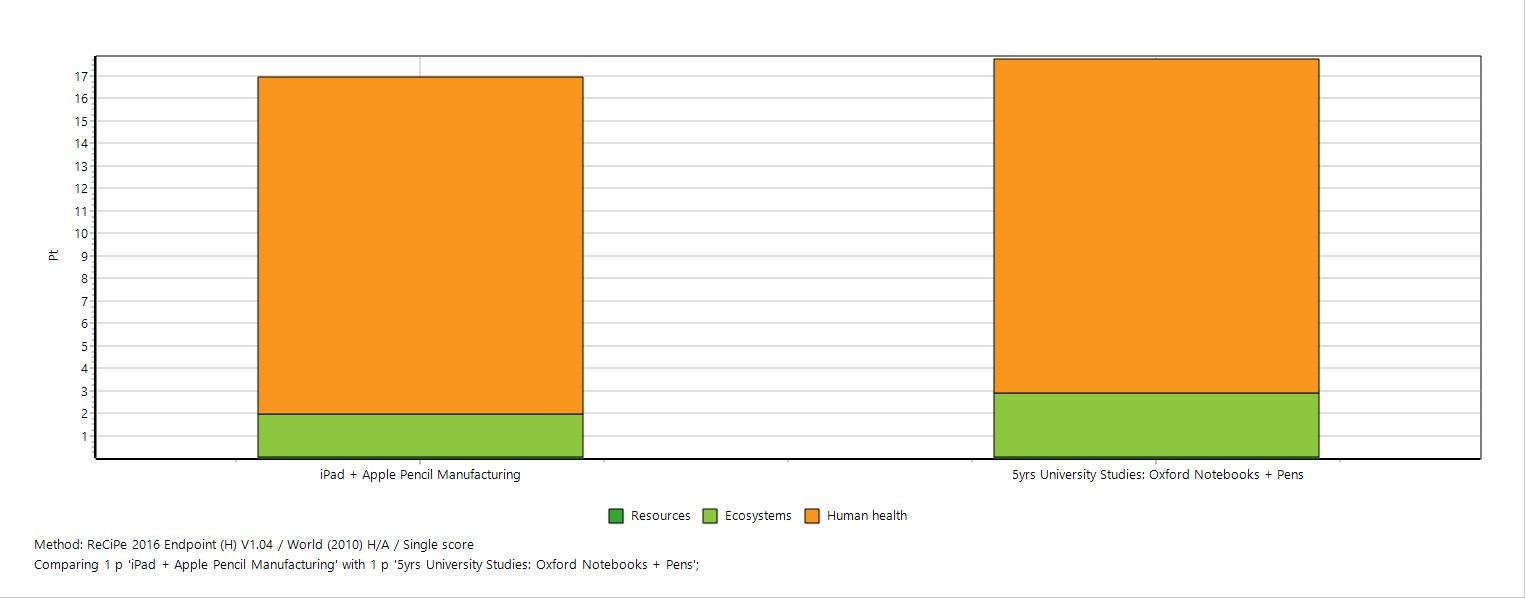
\includegraphics[width=\textwidth]{images/Manufacturing/Single_Score_Manufacturing.JPG}
    \caption{caption}\label{fig:single_score_manufacturing}
\end{figure}


\subsection{Life Cycle Impact}\label{subsec:results_life_cycle}

\subsubsection{0\% RES Penetration}

\begin{figure}[H]
    \centering
    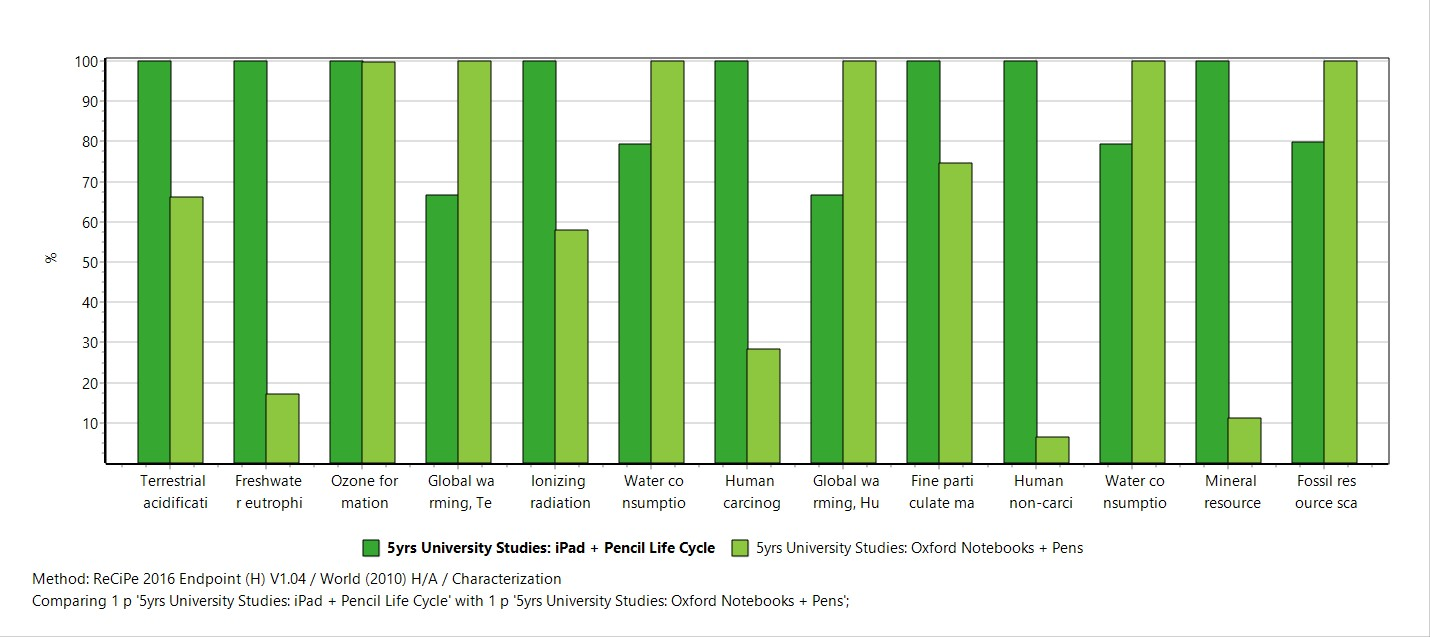
\includegraphics[width=\textwidth]{images/RES_0/Characterization_RES_0.JPG}
    \caption{Relative characterization for a 0\% RES penetration scenario of the investigated note-taking approaches per impact category.}\label{fig:characterization_RES_0}
\end{figure}

\begin{figure}[H]
    \centering
    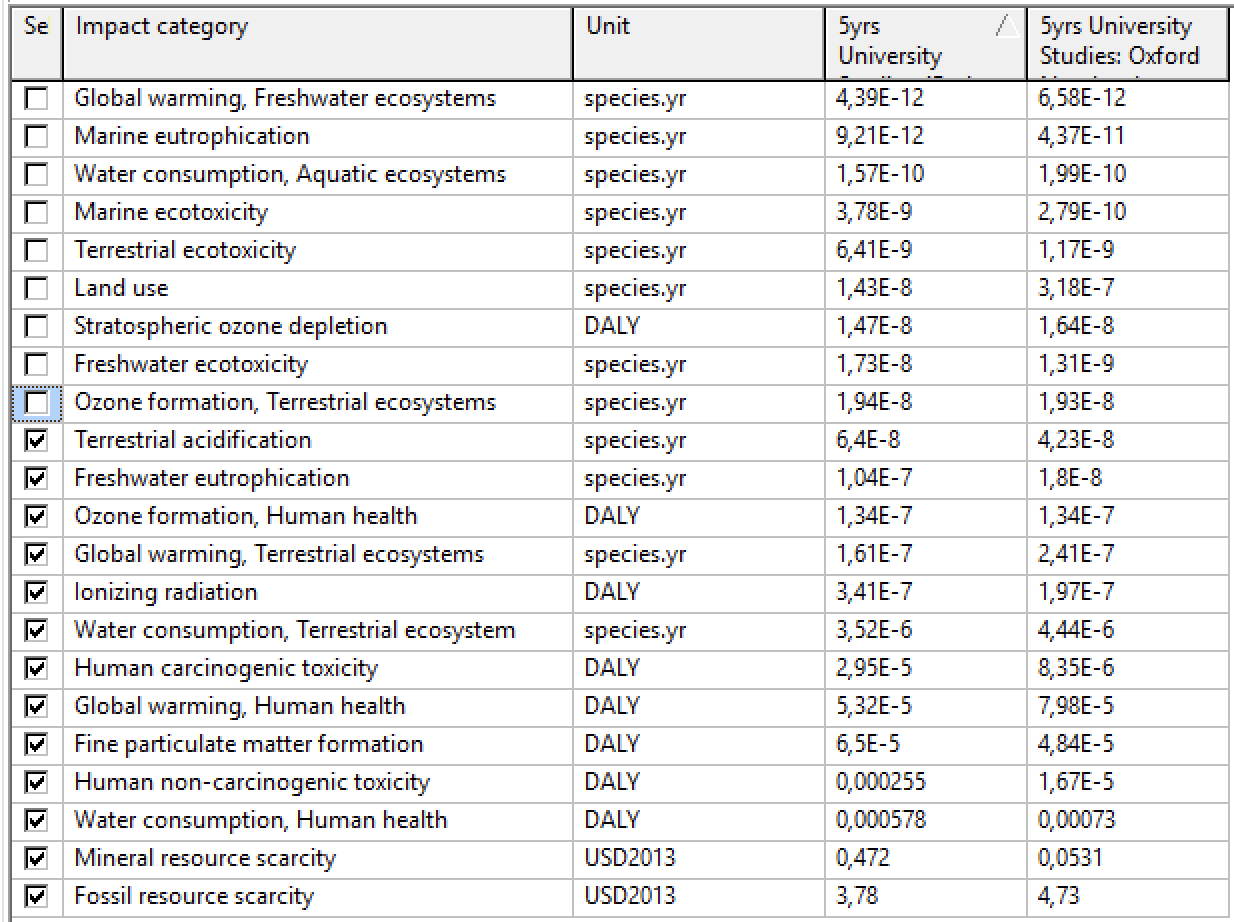
\includegraphics[width=0.9\textwidth]{images/RES_0/Characterization_Table_RES_0.PNG}
    \caption{Absolute characterization for a 0\% RES penetration scenario of the investigated note-taking approaches per impact category.}\label{fig:characterization_table_RES_0}
\end{figure}

\begin{figure}[H]
    \centering
    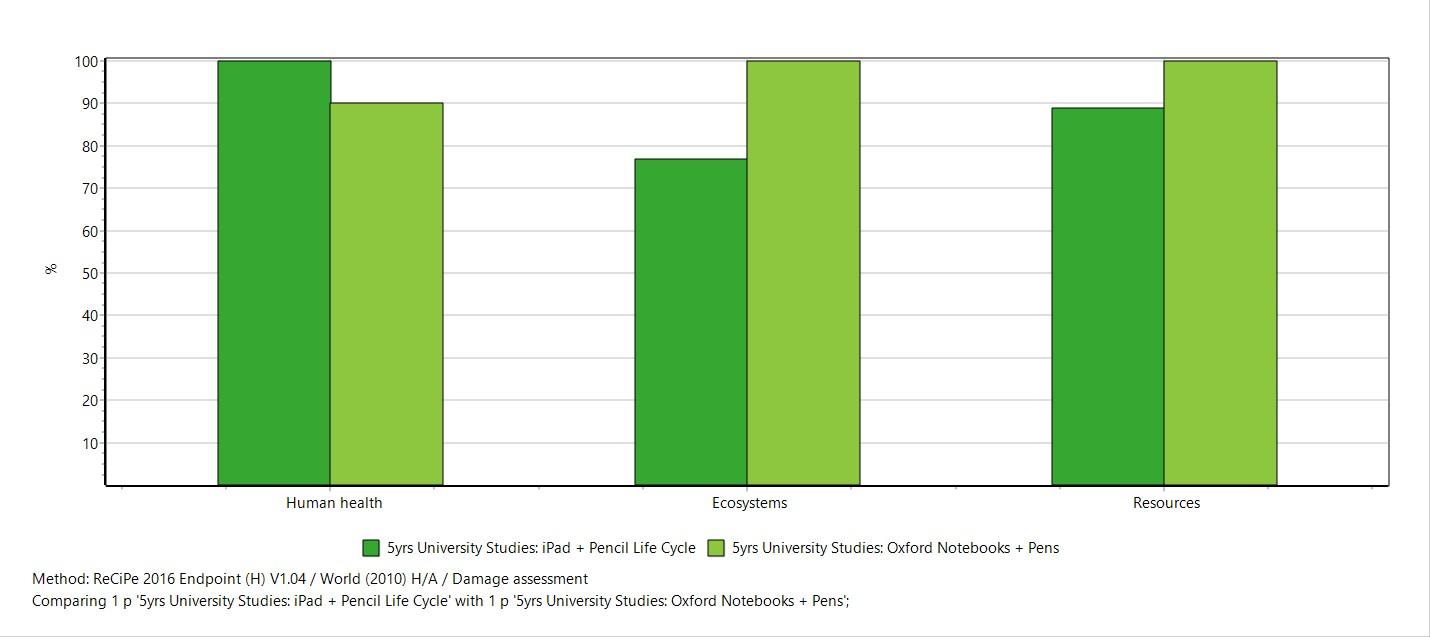
\includegraphics[width=\textwidth]{images/RES_0/Damage_Assessment_RES_0.JPG}
    \caption{caption}\label{fig:damage_assessment_RES_0}
\end{figure}

\begin{figure}[H]
    \centering
    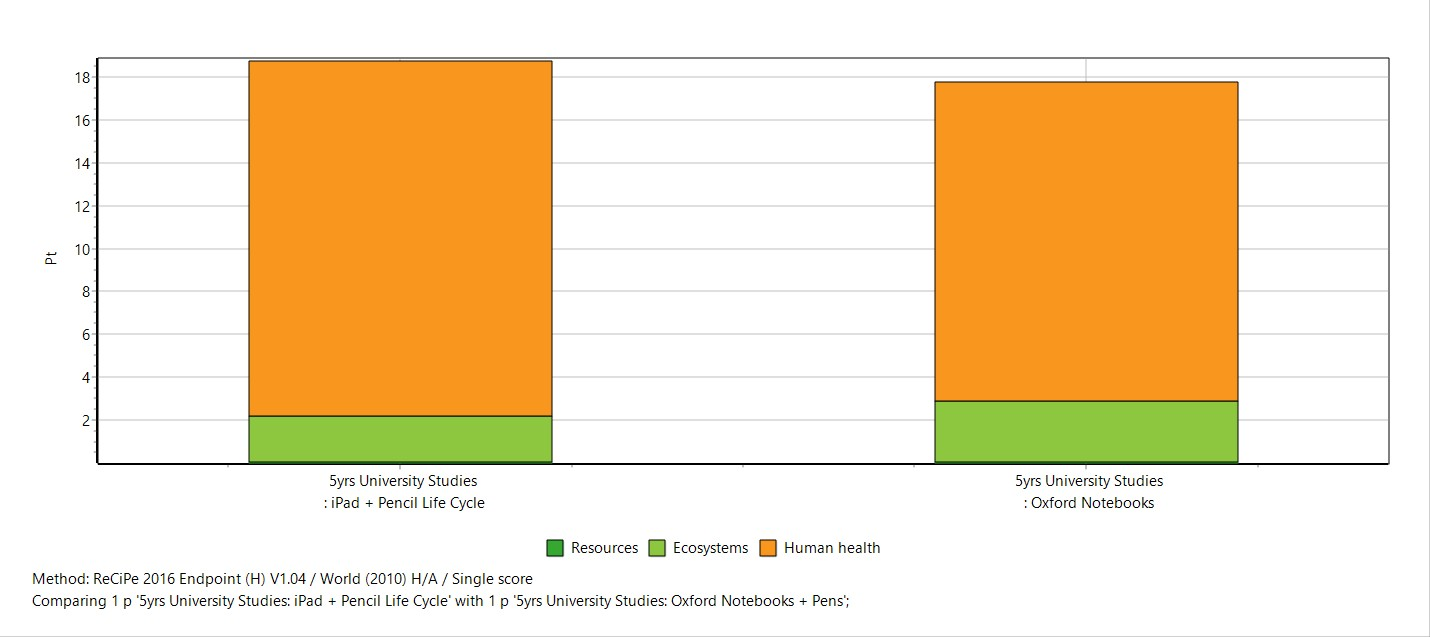
\includegraphics[width=\textwidth]{images/RES_0/Single_Score_RES_0.JPG}
    \caption{caption}\label{fig:single_score_RES0}
\end{figure}

\subsubsection{50\% RES Penetration}

\begin{figure}[H]
    \centering
    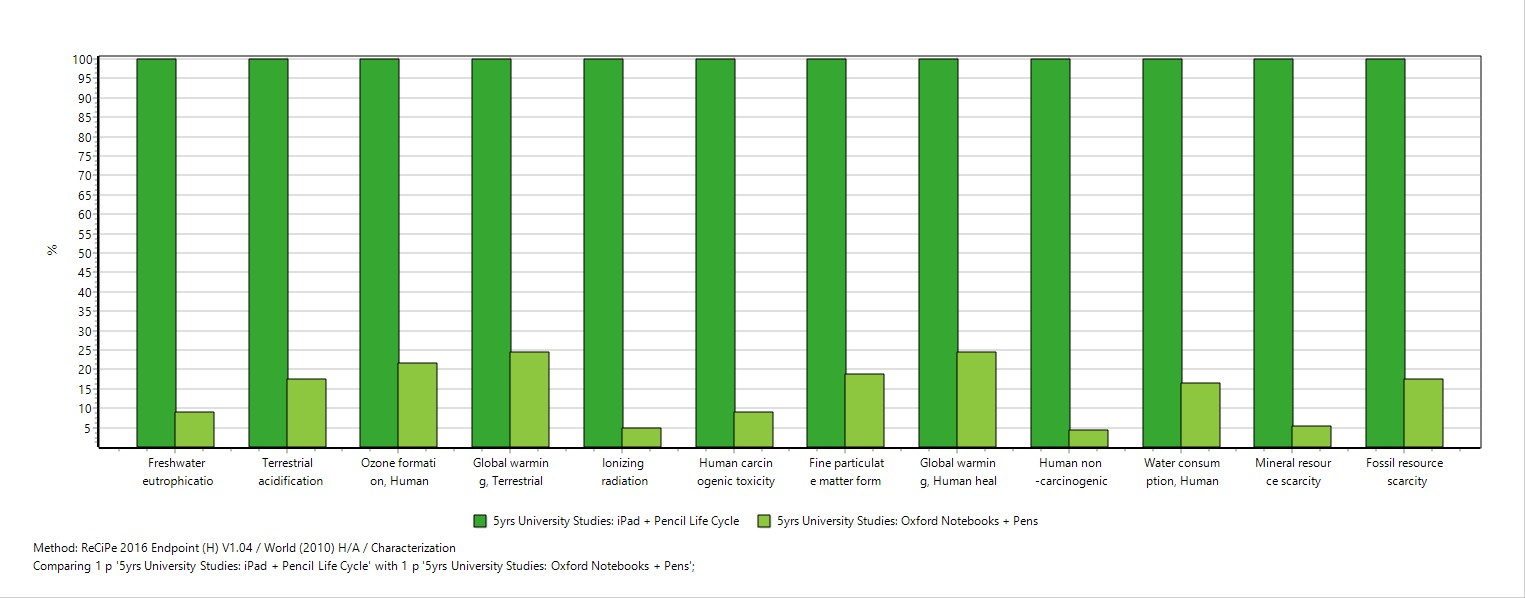
\includegraphics[width=\textwidth]{images/RES_50/Characterization_RES_50.JPG}
    \caption{Relative characterization for a 50\% RES penetration scenario of the investigated note-taking approaches per impact category.}\label{fig:characterization_RES_50}
\end{figure}

\begin{figure}[H]
    \centering
    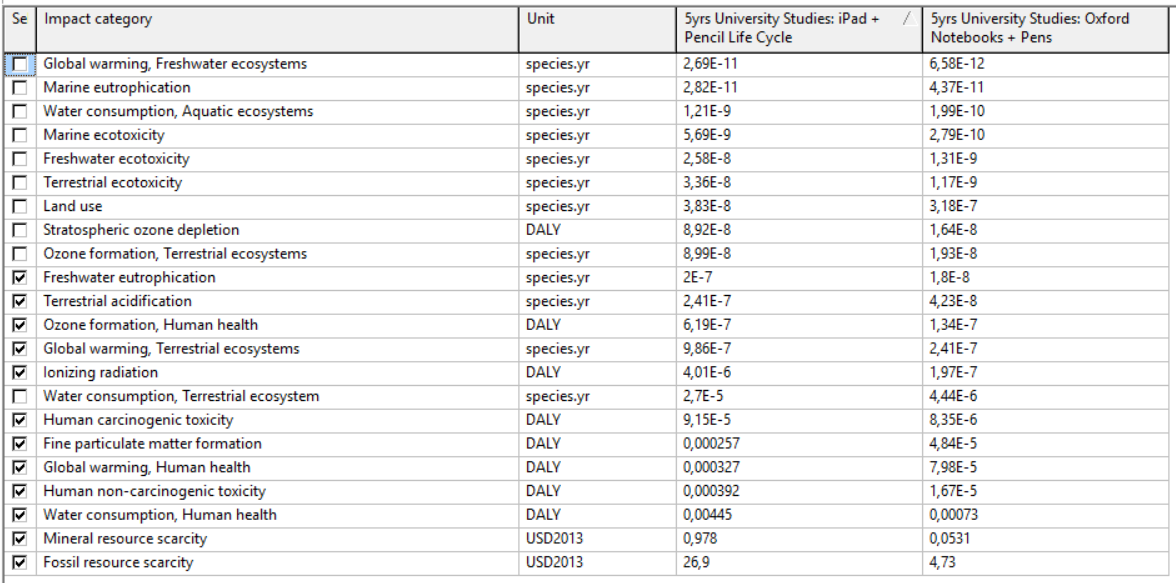
\includegraphics[width=0.9\textwidth]{images/RES_50/Characterization_Table_RES_50.PNG}
    \caption{Absolute characterization for a 50\% RES penetration scenario of the investigated note-taking approaches per impact category.}\label{fig:characterization_table_RES_50}
\end{figure}

\begin{figure}[H]
    \centering
    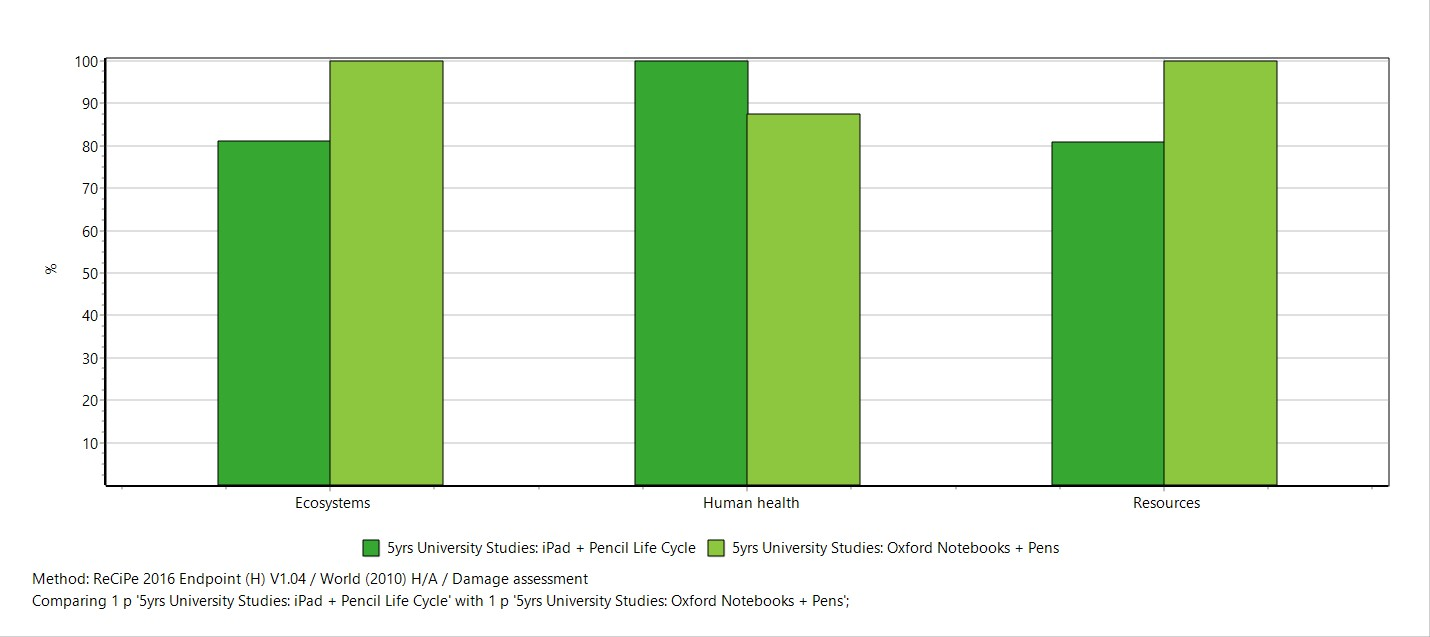
\includegraphics[width=\textwidth]{images/RES_50/Damage_Assessment_RES_50.JPG}
    \caption{caption}\label{fig:damage_assessment_RES_50}
\end{figure}

\begin{figure}[H]
    \centering
    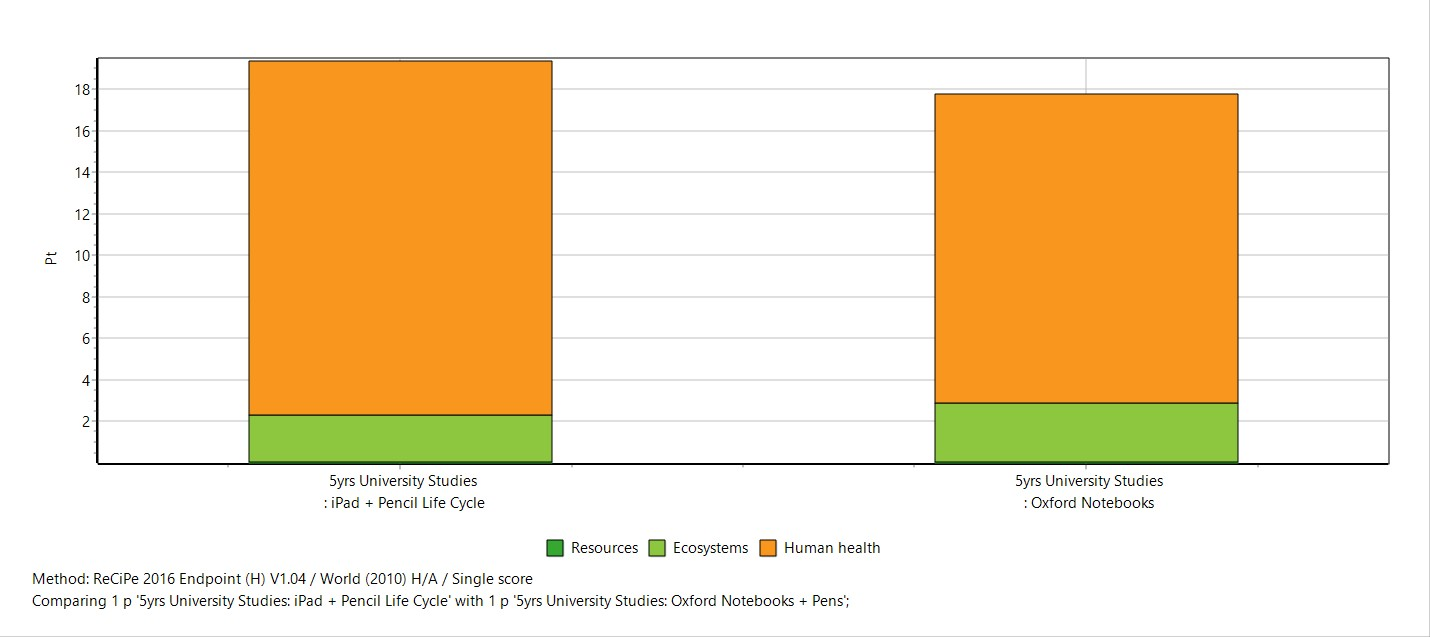
\includegraphics[width=\textwidth]{images/RES_50/Single_Score_RES_50.JPG}
    \caption{caption}\label{fig:single_score_RES50}
\end{figure}

\subsubsection{100\% RES Penetration}

\begin{figure}[H]
    \centering
    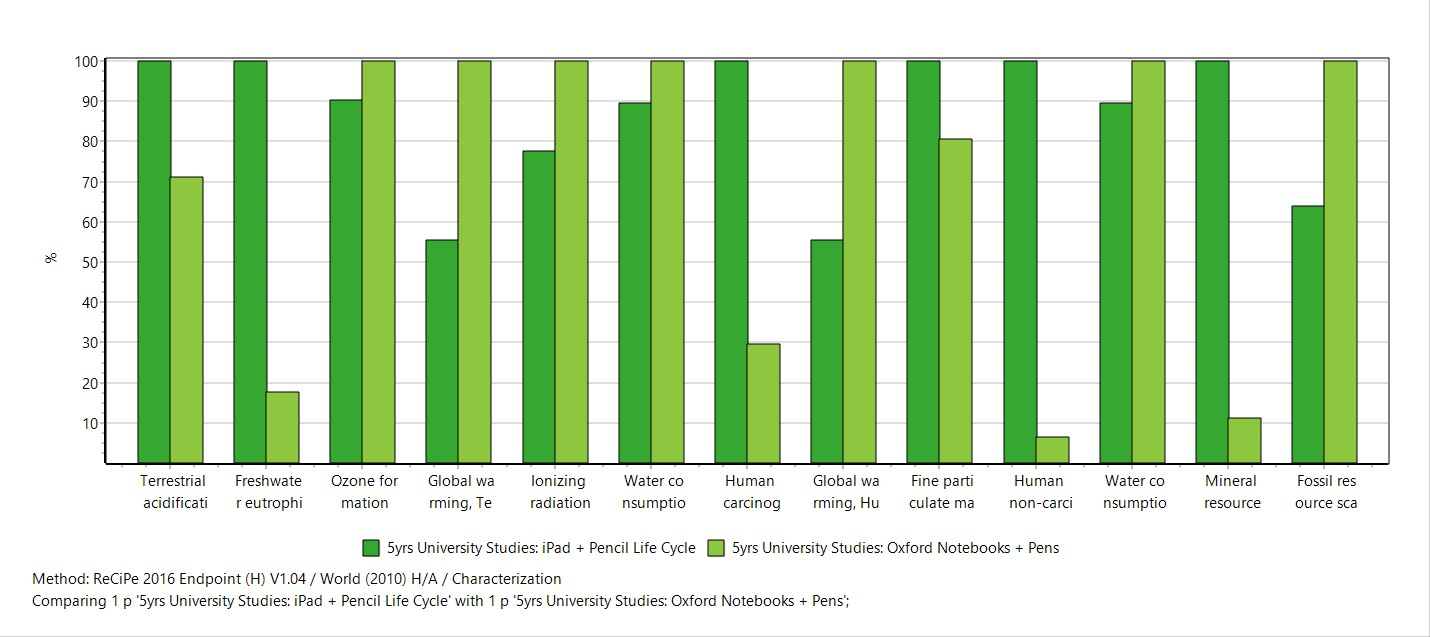
\includegraphics[width=\textwidth]{images/RES_100/Characterization_RES_100.JPG}
    \caption{Relative characterization for a 100\% RES penetration scenario of the investigated note-taking approaches per impact category.}\label{fig:characterization_RES_100}
\end{figure}

\begin{figure}[H]
    \centering
    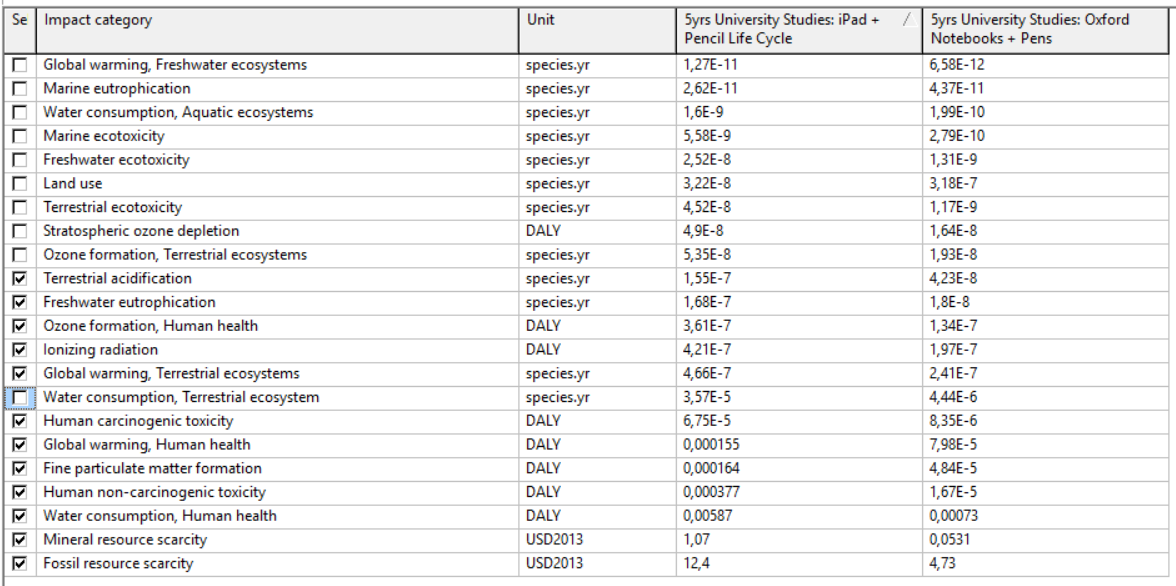
\includegraphics[width=0.9\textwidth]{images/RES_100/Characterization_Table_RES_100.PNG}
    \caption{Absolute characterization for a 100\% RES penetration scenario of the investigated note-taking approaches per impact category.}\label{fig:characterization_table_RES_100}
\end{figure}

\begin{figure}[H]
    \centering
    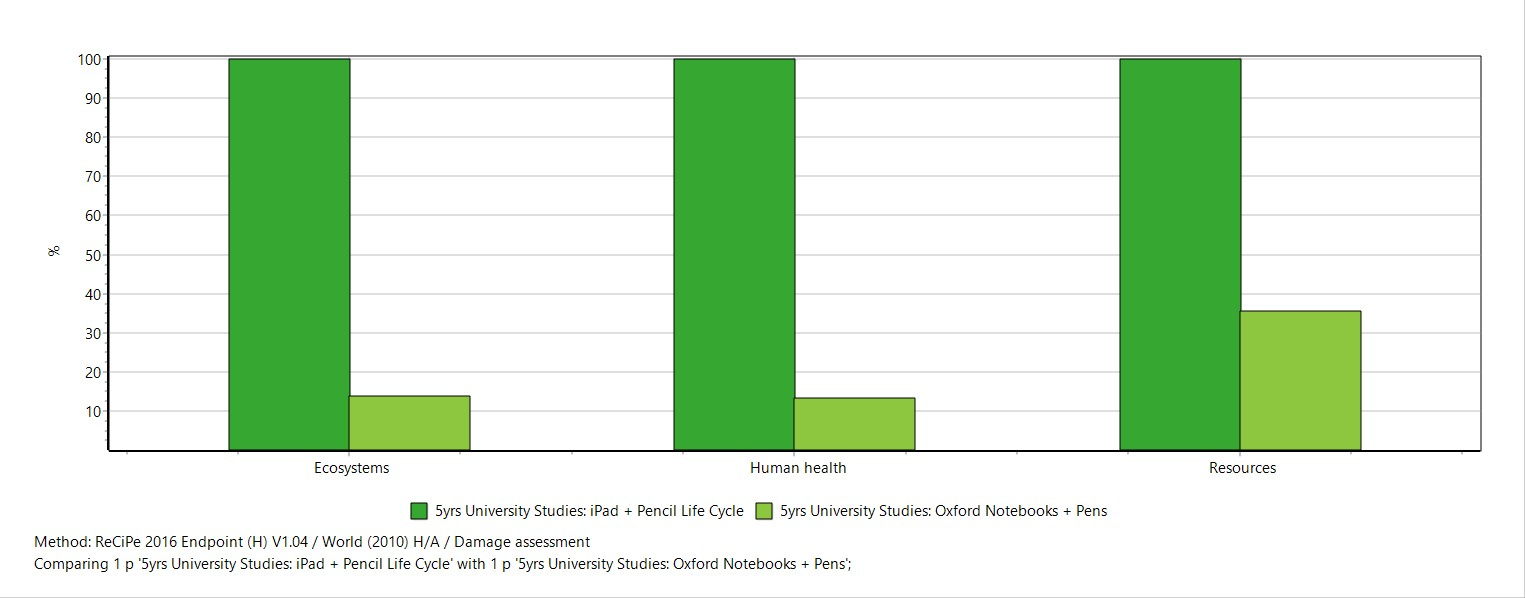
\includegraphics[width=\textwidth]{images/RES_100/Damage_Assessment_RES_100.JPG}
    \caption{caption}\label{fig:damage_assessment_RES_100}
\end{figure}

\begin{figure}[H]
    \centering
    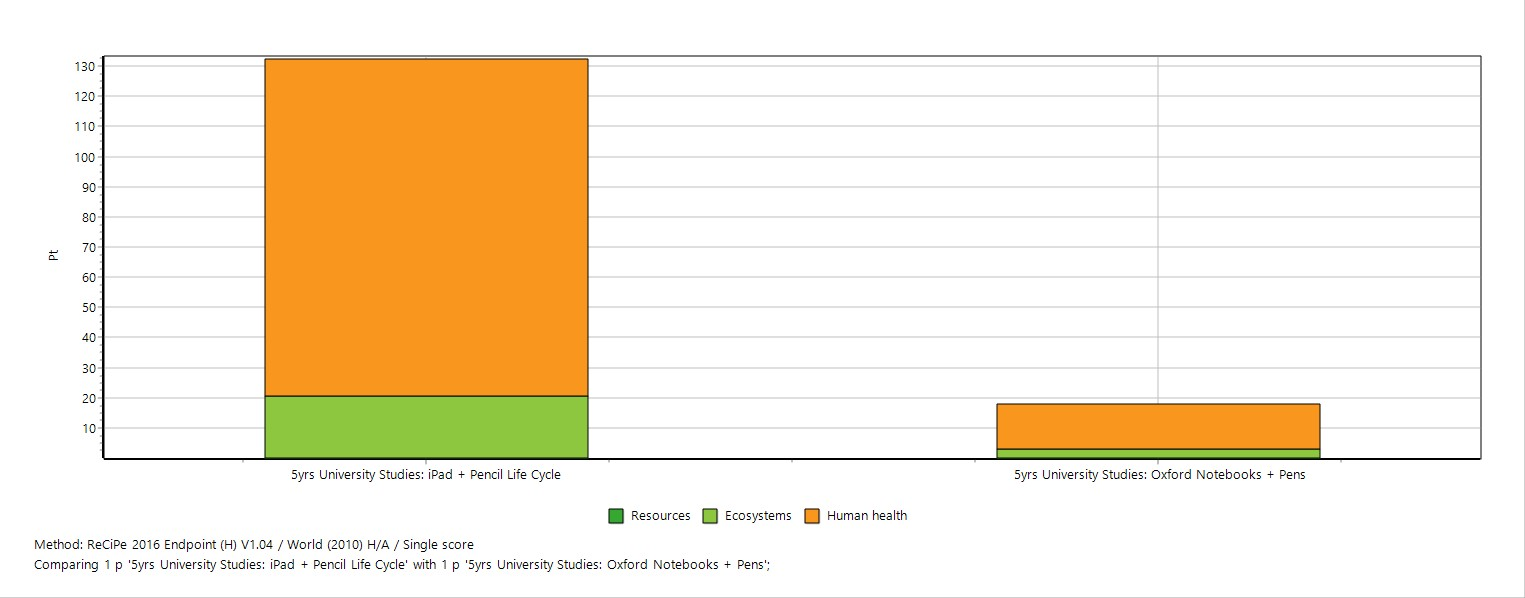
\includegraphics[width=\textwidth]{images/RES_100/Single_Score_RES_100.JPG}
    \caption{caption}\label{fig:single_score_RES100}
\end{figure}